\loesung{
\begin{enumerate}[a)]
  \item Calculation of Pearson correlation coefficient of $x_1$ and $x_2$
  $$
 \rho(x_1, x_2) = \frac{\sum_{i = 1}^n (x_1^{(i)} - \overline{x}_1)(x_2^{(i)} - \overline{x}_2)}{\sqrt{\sum_{i = 1}^n (x_1^{(i)} - \overline{x}_1)^2} \sqrt{\sum_{i = 1}^n (x_2^{(i)} - \overline{x}_2)^2}}
  $$ 
   
  given the dataset:

 \begin{table}[ht]
\centering
\begin{tabular}{rrrrrrrrrr|r}
\hline
& 1 & 2 & 3 & 4 & 5 & 6 & 7 & 8 & 9 & $\sum_{i = 1}^n$ \\ 
\hline
y & -7.79 & -5.37 & -4.08 & -1.97 & 0.02 & 2.05 & 1.93 & 2.16 & 2.13 & -10.92\\ 
$x_1$ & -1.00 & -0.75 & -0.50 & -0.25 & 0.00 & 0.25 & 0.50 & 0.75 & 1.00 & 0 \\ 
$x_2$ & 0.95 & 0.57 & 0.29 & -0.03 & 0.02 & 0.08 & 0.23 & 0.54 & 0.98 & 3.63 \\ 
\hline
\end{tabular}
\end{table}
 
The individual differences to the means are:
 
\begin{table}[H]
\centering
\begin{tabular}{rrrrrrrrrr}
  \hline
 & 1 & 2 & 3 & 4 & 5 & 6 & 7 & 8 & 9  \\ 
\hline
  $x_1^{(i)} - \overline{x}_1$ & -1.00 & -0.75 & -0.50 & -0.25 & 0.00 & 0.25 & 0.50 & 0.75 & 1.00 \\ 
  $x_2^{(i)} - \overline{x}_2$ & 0.55 & 0.17 & -0.11 & -0.43 & -0.38 & -0.32 & -0.17 & 0.14 & 0.58 \\ 
   \hline
\end{tabular}
\end{table}

Then:
     $$ 
    \begin{aligned}
  \rho(x_1, x_2) & = \frac{\sum_{i = 1}^n (x_1^{(i)} - \overline{x}_1)(x_2^{(i)} - \overline{x}_2)}{\sqrt{\sum_{i = 1}^n (x_1^{(i)} - \overline{x}_1)^2} \sqrt{\sum_{i = 1}^n (x_2^{(i)} - \overline{x}_2)^2}} \\
  & = \frac{-0.574 + -0.125 + 0.057 + 0.108 + 0 + -0.081 + -0.087 + 0.103 + 0.577}{2.086} = \frac{0.05}{2.086} = 0.002
    \end{aligned}
  $$ 
  
  The Pearson correlation coefficient is close to 0. $\Rightarrow$ There is \textbf{no linear} relationship between $x_1$ and $x_2$, and they are not linearly correlated.
  
  \item  The scatter plot reveals that there is a strong non-linear/quadratic relationship between $x_1$ and $x_2$. The Pearson correlation coefficient is not suitable for detecting non-linear relationships.
  
	\begin{center}
	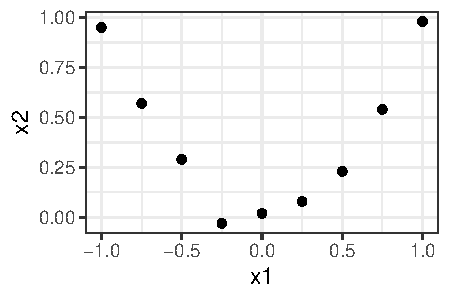
\includegraphics[width=1.3\maxwidth]{figure/add_Points_x1_x2_sol.pdf}
	\end{center}

  %  \item The p-value (for estimating the GAM) of $2.79 \times 10^{-5}$ (but also the adjusted $R^2$ value) reveals that there is a strong relationship between $x_1$ and $x_2$.
  %  But: The p-value does not reveal the shape of this relationship.

  % \item[$\Rightarrow$] More suitable: \textbf{Mutual Information (MI)}

  \item The \textbf{mutual information (MI)} is more suitable for this data distribution. The formula for the mutual information is:
  
  \begin{equation}\label{eq:def_mutual_information}
  	MI(x_1 ; x_2 ) =  \mathbb{E}_{p(x_1, x_2)} \left[ \log\left(\frac{p(x_1, x_2)}{p(x_1) p(x_2)} \right) \right] = \sum_{x_1} \sum_{x_2} p(x_1, x_2) \log\left(\frac{p(x_1, x_2)}{p(x_1) p(x_2)} \right)
  \end{equation}
  
  % Problem: distribution needed. \\
  Problem: We need a distribution, because the MI is defined using an expected value.
  This expected value can only be evaluated directly if we explicitly know the distribution of the data (which we do not in this case).
  If we simply use the empirical form (the sum in formula \eqref{eq:def_mutual_information}) and plug in the 9 data points from above, we will obtain a very high MI, because we have too few samples. It would erroneously indicate an extremely strong dependency, but is not very informative in this case.
  
  We therefore first have to estimate the whole distribution from our data points, and can then calculate the MI for this estimated distribution, which is an approximation of the true MI. \\
  This approximation becomes better and better, the more data points one samples.
  
\end{enumerate}
}

\dlz

\bonusloesung{

  One possible solution: Estimate the distribution using histograms with Gaussian kernel. This practically means: We split the ranges of the features into intervals (buckets) and calculate the empirical distributions w.r.t. these buckets:
  \begin{center}
  	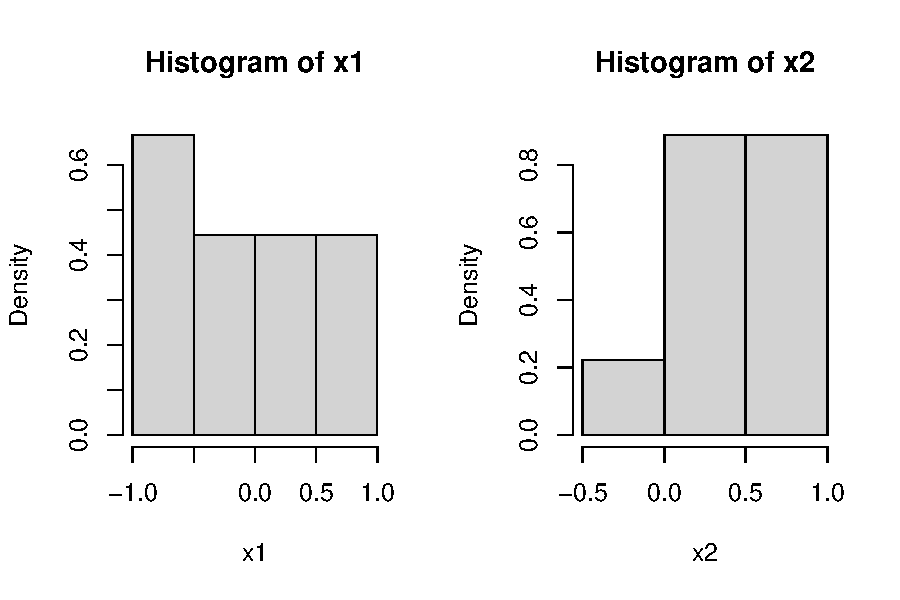
\includegraphics[width=0.79\maxwidth]{figure/hist_x1_x2.pdf}
  \end{center}
  Now, we take the mean values as replacement for the values in $x_1$ and $x_2$:
  \begin{table}[H]
  	\centering
  	\begin{tabular}{r|rrrrrrrrr}
  		\hline
  		& 1 & 2 & 3 & 4 & 5 & 6 & 7 & 8 & 9 \\ 
  		\hline
  		$x_1^\star$ & -0.75 & -0.75 & -0.75 & -0.25 & -0.25 & 0.25 & 0.25 & 0.75 & 0.75 \\ 
  		$x_2^\star$ & 0.75 & 0.75 & 0.25 & -0.25 & 0.25 & 0.25 & 0.25 & 0.75 & 0.75 \\ 
  		\hline
  	\end{tabular}
  \end{table}  
  Equivalently, one could also introduce categories for the single intervals and make \(x_1\) and \(x_2\) categorical variables.
  We then compute the table with joint and marginal distribution: 
  \begin{table}[H]
  	\centering
  	\begin{tabular}{r|rrr|r}
  		\hline
  		$x_2^\star$ & -0.25 & 0.25 & 0.75 & $p_{x_1}$ \\ 
  		\hline
  		$x_1^\star$ \hspace*{0.2cm} -0.75 & 0.00 & 0.11 & 0.22 & 0.33 \\ 
  		-0.25 & 0.11 & 0.11 & 0.00 & 0.22 \\ 
  		0.25 & 0.00 & 0.22 & 0.00 & 0.22 \\ 
  		0.75 & 0.00 & 0.00 & 0.22 & 0.22 \\
  		\hline 
  		$p_{x_2}$& 0.11 & 0.44 & 0.44 & 1.00 \\ 
  		\hline
  	\end{tabular}
  \end{table}
Now we can calculate the MI for this approximate distribution, which is very close to the MI of our original distribution: 
   \begin{align*}
   	MI(x_1^\star ; x_2^\star) = & \sum_{x_1^\star} \sum_{x_2^\star} p(x_1^\star, x_2^\star) \, \log\left(\frac{p(x_1^\star, x_2^\star)}{p(x_1^\star) p(x_2^\star)} \right)\\
 	= & \,0\, \log\left(\frac{0}{0.33 \cdot 0.11} \right) 
   	+ 0.11\, \log\left(\frac{0.11}{0.33 \cdot 0.44} \right) 
   	+ 0.22\, \log\left(\frac{0.22}{0.33 \cdot 0.44} \right) \\
   	& + 0.11\, \log\left(\frac{0.11}{0.22 \cdot 0.11} \right)
   	+ 0.11\, \log\left(\frac{0.11}{0.22 \cdot 0.44} \right) 
   	+ 0\, \log\left(\frac{0}{0.22 \cdot 0.44} \right) \\
   	& + 0\, \log\left(\frac{0}{0.22 \cdot 0.11} \right)
   	+ 0.22\, \log\left(\frac{0.22}{0.22 \cdot 0.44} \right) 
   	+ 0\, \log\left(\frac{0}{0.22 \cdot 0.44} \right) \\
   	& + 0\, \log\left(\frac{0}{0.22 \cdot 0.11} \right)
   	+ 0\, \log\left(\frac{0}{0.22 \cdot 0.44} \right) 
   	+ 0.22\, \log\left(\frac{0.22}{0.22 \cdot 0.44} \right) \\
   	\approx & \, 0.603
   \end{align*}
$\Rightarrow$
The MI of around 0.6 shows that there is a clear dependency.

}
